\chapter{User Manual}
\label{manual}

This is the user manual for caxap, a macro system layered on top of
Java. Although there are references to other parts of this thesis, the manual is
designed to stand on his own as much as possible. The manual specifically
targets would-be users of our macro system.

This manual assumes that you, the user, are familiar with the notion of
\emph{tree} in computer science. This means you should be able to understand
concepts such as \emph{node}, \emph{leaf}, \emph{root}, \emph{child},
\emph{parent}, \emph{depth} and \emph{depth-first walk} in the context of
trees. If you are not, you can learn about trees on wikipedia (*) or elsewhere.

(*) \url{http://en.wikipedia.org/wiki/Tree_(data_structure)}

We also assume that you are familiar with the PEG formalism, which is described
in chapter \ref{peg_intro} of this thesis. Sections \ref{peg_formalism} and
\ref{extended_notation} form a self-contained definition of the PEG notation
used in caxap.

\emph{caxap} means \emph{sugar} in russian. It should be pronounced ``katchap''.
(This is not the correct russian pronunciation, which sounds more like
``zehrer''.) The name was chosen because caxap adds syntactic sugar on top of
Java.

%%%%%%%%%%%%%%%%%%%%%%%%%%%%%%%%%%%%%%%%%%%%%%%%%%%%%%%%%%%%%%%%%%%%%%%%%%%%%%%%
\section{Introduction}

This section introduces caxap's fundamentals. Do not skip over it, as it
contains crucial information not repeated later on.

%%%%%%%%%%%%%%%%%%%%%%%%%%%%%%%%%%%%%%%%%%%%%%%%%%%%%%%%%%%%%%%%%%%%%%%%%%%%%%%%
\subsection{What is \emph{caxap} ?}

caxap is a macro system for the Java language. More accurately, it is a Java
source preprocessor that expands user-defined macros. caxap is unique in that it
allows macros to have arbitrary user-defined syntax.

%%%%%%%%%%%%%%%%%%%%%%%%%%%%%%%%%%%%%%%%%%%%%%%%%%%%%%%%%%%%%%%%%%%%%%%%%%%%%%%%
\subsection{What is a macro?}

In caxap, a macro is a new syntactic construct you add to the language. When you
define a macro, you have to supply three pieces of information.

First, what the syntax will look like. We call this \emph{the syntactic
  specification}.

Second you need to specify how this new syntax will be translated into old
syntax. This is done in the \emph{the macro body}. The macro body contains the
\emph{expansion code}. Old syntax comprises the base Java language, and any
macros that might have been defined beforehand.

Third, you need to specify where the macro can appear. You do this by giving the
name of a grammar rule. The macro's syntactic specification will be added as an
alternative for that rule.

%%%%%%%%%%%%%%%%%%%%%%%%%%%%%%%%%%%%%%%%%%%%%%%%%%%%%%%%%%%%%%%%%%%%%%%%%%%%%%%%
\subsection{How does caxap deal with files?}

This is a simplified overview of the whole process. We fill in the details later
on. We use the term \emph{source file} to designate both \emph{regular source
  files} (\texttt{.java}) and \emph{macro files} (\texttt{.javam}).

The first thing caxap does is examine the source directories and find all macro
files that live (directly or indirectly) under those directories. Each source
file may depend on other source files. caxap traces these dependencies and
ensures that the resulting graph does not contain any loop, else the process
cannot continue. caxap then proceeds to compile the macros and all classes they
depend on, expanding the macro calls in them as needed. Once this is done, caxap
is equipped with the knowledge required to expand all remaining macro calls it
could encounter. caxap now considers all regular sources files that have not yet
been processed, and proceeds to expand their macro calls. The expansions of all
regular source files are then placed under the output directory, in a way that
mimics the original source directory trees. If a file contains no macro calls,
it is nevertheless copied to the output directory.

The next step is to use your usual Java compiler to compile the expanded
sources. caxap is not involved in that step.

%%%%%%%%%%%%%%%%%%%%%%%%%%%%%%%%%%%%%%%%%%%%%%%%%%%%%%%%%%%%%%%%%%%%%%%%%%%%%%%%
\subsection{How does caxap recognize macros?}

This section explains succinctly how caxap is able to recognize macros with
arbitrary syntax.

To parse source files, caxap relies on parsing expression grammars (PEGs). A
grammar is a precise definition of language's syntax. If you are not familiar
with formal grammars, you might want to read chapter \ref{peg_intro} before
proceeding.

In caxap, all rules are implicitly also choices. This allows us to enable or
disable macros without changing the structure of the grammar each time; simply
by adding or removing an \emph{alternative} to a rule.

When you define a new macro, you need to specify the syntax using the PEG
notation. This forms the macro's syntactic specification. The specification is
used to make a new PEG rule. This rule is added to the grammar as an alternative
to an existing rule. You can choose the rule that your macro's own rule should
be an alternative of.

Macro definitions are encountered while parsing. After parsing a macro
definition, this definition is processed. As a result, a rule corresponding to
the syntactic specification is added to the grammar; before parsing the rest of
the file. This means that the grammar does actually change while we are parsing!

When parsing a file, the base grammar is the Java grammar, with some additions
that enables importing and defining macros. This grammar is reproduced in
appendix \ref{grammar}. Macros can be \emph{required} (imported) within
files. Requiring a macro causes its rule to be added to the grammar used to
parse the file.

%%%%%%%%%%%%%%%%%%%%%%%%%%%%%%%%%%%%%%%%%%%%%%%%%%%%%%%%%%%%%%%%%%%%%%%%%%%%%%%%
\subsection{How does caxap expand macros?}
\label{macro_expansion_intro}

After recognizing a macro call, caxap is in possession of its syntax tree, based
on the macro's syntatic specification. caxap then invokes the expansion code
from the macro's body, passing it the syntax tree. The expansion code returns a
replacement syntax tree. This syntax tree is itself checked for macro
calls. Found calls are expanded, and this process continues until the
replacement is free of macro calls. Note that if the user is not careful, he can
cause an infinite loop by writing a macro that expands to itself.

Said otherwise, macros are recursively expanded up to the obtention of a fixed
point: the point where there are no more macros to expand.

We say that macros are \emph{recursively expanded} to describe this expansion
mechanism. Note that macros are also recursive in the sense that a macro body
can contain macro calls which are expanded before compiling the macro. However,
A macro cannot, directly or indirectly use itself in its expansion code.

%%%%%%%%%%%%%%%%%%%%%%%%%%%%%%%%%%%%%%%%%%%%%%%%%%%%%%%%%%%%%%%%%%%%%%%%%%%%%%%%
\subsection{Where can macro calls appear?}

Macro calls may not appear among, or directly after \texttt{import} and
\texttt{require} statements. A known construct needs to be encountered following
those statements before macro can be processed. Other than that, macro calls can
appear anywhere.

\texttt{require} statements are described in section \ref{require_manual} of
this manual.

In macro files, macros whose definition is the result of a macro expansion are
not available for use in the same file.

%%%%%%%%%%%%%%%%%%%%%%%%%%%%%%%%%%%%%%%%%%%%%%%%%%%%%%%%%%%%%%%%%%%%%%%%%%%%%%%%
\section{Installation}

Running caxap requires the Java Development Kit (JDK) version 7.

You can obtain caxap online at \url{https://github.com/norswap/caxap}. This page
explains how to compile caxap and how to obtain a precompiled JAR
file. Compilation uses the Apache Maven build system.

Once you have a caxap's JAR file handy, you can use it as described in the next
section.

%%%%%%%%%%%%%%%%%%%%%%%%%%%%%%%%%%%%%%%%%%%%%%%%%%%%%%%%%%%%%%%%%%%%%%%%%%%%%%%%
\section{Invocation}

\texttt{java [<java_options>] -jar <caxap_jar> [<options>]}

For instance, \texttt{<caxap_jar>} could be \texttt{caxap-1.0.jar}. No option is
mandatory. Here is a listing of valid options:

\begin{itemize}

\item \texttt{-charset <charset>} : Changes the charset used to parse the source
  files. A list of valid charset names can be found in the Javadoc for the
  standard library \texttt{Charset} class
  (\url{http://docs.oracle.com/javase/7/docs/api/java/nio/charset/Charset.html})
  . Defaults to UTF-8.

\item \texttt{-source <directory>} : Indicates the the given directory contains
  source files. Multiple such options can be provided. If none are, defaults to
  \texttt{src}.

\item \texttt{-output <directory>} : Indicates the directory under which caxap
  should write the macro-expanded code. This will be the source directory for
  the compiler run after caxap. Defaults to \texttt{generated}.

\item \texttt{-cache <boolean>} : If \texttt{true}, caxap will output the
  bytecode for source files it compiles itself (including macros) under the
  binary directory. In the future, this will also control whether caxap should
  recompile source files which haven't changed (much like how the \emph{make}
  program works). Defaults to \texttt{true}.

\item \texttt{-binary <directory>} : Indicates the directory under which caxap
  should write the \texttt{.class} files if the cache option is set to
  \texttt{true}. Defaults to \texttt{target/classes}.

\item \texttt{-dump <boolean>} : If \texttt{true}, caxap will output
  macro-expanded version of macro files under the output directory. Defaults to
  \texttt{true}.

\end{itemize}

In the options description, when we say that a directory contains source files,
or that source files will be written under a directory; we assume that the
package structure is respected. The relative path of a class containing the
definition of the public class \texttt{something.stuff.MyClass} should be
\texttt{something/stuff/MyClass.java}.

%%%%%%%%%%%%%%%%%%%%%%%%%%%%%%%%%%%%%%%%%%%%%%%%%%%%%%%%%%%%%%%%%%%%%%%%%%%%%%%%
\section{A Simple Example}
\label{simple_example}

Figure \ref{simple_macro_example} show a very simple macro, how it can be used,
and the resulting expansion. The defined construct is an \emph{unless}
statement. It takes an expression and a statement, and executes the statement
only if the supplied expression evaluates to false.

You can find the sources for this example - as well as others - under the
\texttt{examples} directory in the caxap source repository. The
\texttt{examples/README.md} file indicates how to run the examples for
yourself. The syntax has been slightly reformatted to fit the printed page,
especially the expanded source, since that is not currently pretty-printed by
caxap.

\begin{figure}[here]
\small
\begin{lstlisting}[language=Java, frame=single]
// src/pkg/Use.java

package pkg;
require macro pkg.Unless;

class Use {
  public static void main(String[] args) {
    unless false {
      System.out.println("Hopla boum!");
    }
  }
}

// src/pkg/Unless.javam

package pkg;

macro Unless as statement
: "unless" expr:expression :block {
  return `statement[ if (!(#expr[0])) #block[0] ]`;
}

// generated/pkg/Use.java

package pkg;

class Use {
  public static void main(String[] args) {
    if (!((false))) {
      System.out.println("Hopla boum!");
    }
  }
}

\end{lstlisting}
\caption{caxap code showing how to use and define a simple \emph{unless}
  construct, as well as the Java code resulting from macro expansion.}
\label{simple_macro_example}
\end{figure}

This simple example showcases most important concepts in caxap. Let's examine
the macro definition.

\texttt{Unless} is the macro name. This is the name which is referenced to make
use of the macro in a source file, as shown in the line [\texttt{require macro
  pkg.Unless;}] from \texttt{pkg/Unless.javam}. The macro name is also the name
of the grammar rule associated to the macro.

The [\texttt{as statement}] part tells us two things. The first is that the
macro's grammar rule will be inserted in the grammar as the last alternative for
the rule \texttt{statement}. The second indication is given by the \texttt{as}
keyword. It means that the macro will expand to a \texttt{statement} syntax tree
node, and that this node should replace the \texttt{statement} node matched by
the macro. There are other kinds of expansion strategies, which we describe in
section \ref{expansion_strategies}.

The part between the colon and the opening brace is the macro's syntactic
specification, namely [\lstinline{"unless" expr:expression :block}].

It defines the syntax of our macro, using the PEG notation as described in
sections \ref{peg_formalism} and \ref{extended_notation}. The rules
\texttt{expression} and \texttt{statement} are defined in the base grammar (see
appendix \ref{grammar}).

To the PEG syntax as described previously, we add the \emph{capture} operator:
[\texttt{<name>:<expression>}]. We cover captures in detail in section
\ref{captures_manual}. For now it suffices to know they allow us to capture
parts of the matched syntax tree and easily reference those parts in the macro
body.

The statements between the two braces form the macro body:
[\lstinline|return `statement[ if (!(#expr[0])) { #stmt[0] } ]`;|]

The whole expression between backquotes (\texttt{\`{}}) is called a
quasiquotation. We use it to produce a \texttt{statement} syntax tree node. The
source code for the node is the code between square brackets. The expressions
preceded by a hash sign (\texttt{\#}) reference the captures we made in the
syntactic specification.

This shows that we can easily match some syntax, capture its relevant parts and
inject them in replacement code. caxap does not however limit you to such
schemes. The macro body can indeed contain arbitrary Java code. caxap also comes
with facilities to ease the manipulation of syntax trees. Those facilities are
described in section \ref{match_api}.

Finally, notice that we wrapped our expression is parentheses in
\lstinline{!(#expr[0])}. This is necessary because the \texttt{!} operator
expects an operand that does not contain binary operators. Yet the syntactic
specification references the \texttt{expression} rule. This means that an
expression such as \texttt{myVariable == null} would lead to the interpretation
\texttt{(!myVariable) == null} and break our macro. There are two possible
fixes: use parentheses in the expansion like we did; or reference the
\texttt{prefixOperator} rule to explicitly disallow binary operators. In that
last case, the user can still use binary operators but has to wrap them within
parentheses himself. In practice, caxap's quasiquotation mechanism is able to
detect and warn you about the misinterpretation.

%%%%%%%%%%%%%%%%%%%%%%%%%%%%%%%%%%%%%%%%%%%%%%%%%%%%%%%%%%%%%%%%%%%%%%%%%%%%%%%%
\section{The \texttt{require} Statement: Importing Macros and Specifying
  Dependencies}
\label{require_manual}

Section \ref{simple_example} introduced how macros are used in source files: you
indicate which macros you are going to use with \texttt{require} statements, and
then simply use the required macros' syntax in your sources.

The scope of the \texttt{require} statement is in fact larger. It is used to
specify dependencies between source files - both regular and macro files - at
compile time.

The reason we want to specify dependencies between source files at compile time
is to determine the order in which the files should be compiled. If a regular
source file uses a macro, then the macro's expansion code needs to be compiled
before we are able to compile the source file. Conversely, if a macro's
expansion code contains calls to other macros, or if the expansion code uses
other classes, those should be compiled beforehand. We also need to specify
dependencies between regular source files, in order to obtain the transitive
dependencies on macro files.

When working with files which have to be ordered, the challenge is to avoid
dependencies loops. Section \ref{why_source_deps} explains exactly why
dependency loops are not manageable in caxap.

Macros cannot appear among or directly after \texttt{import} and
\texttt{require} statements. caxap does indeed resolve all source dependencies
before starting to compile macros, and it needs to parse a known construct to be
sure that all \texttt{require} statements have been read.

%%%%%%%%%%%%%%%%%%%%%%%%%%%%%%%%%%%%%%%%%%%%%%%%%%%%%%%%%%%%%%%%%%%%%%%%%%%%%%%%
\subsection{\texttt{import} and \texttt{require}}

Also notice we don't use regular \texttt{import} statements to specify
dependencies between sources files. \texttt{import} statement work on classes,
and there isn't a one-to-one mapping between classes and source files. Section
\ref{import_problems} highlights more issues that prevent us from using
\texttt{import} statement for our purpose.

Yet, managing \texttt{require} and \texttt{import} statements separately would
be tedious. This is why the \texttt{require} statements are designed to also
cover the functionality of \texttt{import} statements. In fact, \texttt{require}
statements are replaced by \texttt{import} statements in the expanded source
files, when requiring regular source files.

To do this, the require statement needs to have two bits of information: what we
import, and where we import it from. The next few sections show how
\texttt{require} statements convey that information.

Macros and classes living in the same package as the file are not implicitly
required, whereas classes in the same package are implicitly imported.

%%%%%%%%%%%%%%%%%%%%%%%%%%%%%%%%%%%%%%%%%%%%%%%%%%%%%%%%%%%%%%%%%%%%%%%%%%%%%%%%
\subsection{General Form}

In its general form, a require statement consists of two qualified identifiers
separated by a colon. A qualified identifier is a dot-separated list of
identifiers. For instance:

\texttt{require com.company.project.Class:Class.Nested;}

The identifier immediately preceding the colon (\texttt{Class}) is the stem of a
filename; that of the file depended upon (\texttt{Class.java}). The identifiers
that precede this identifier form the package name
(\texttt{com.company.project}). This gives us the file position:
\texttt{com/company/project/Class.java}.

From that file, we want to import the item designed by the second qualified
identifier (\texttt{Class.Nested}). We want the nested class \texttt{Nested}
which lives under the top-level class \texttt{Class}.

Just like with \texttt{import} statements, you can't import things from the
default package.

The next few sections detail variants of the general form. A formal
specification of the full syntax of \texttt{require} statements can be found in
section \ref{requires_grammar} of the appendices.

%%%%%%%%%%%%%%%%%%%%%%%%%%%%%%%%%%%%%%%%%%%%%%%%%%%%%%%%%%%%%%%%%%%%%%%%%%%%%%%%
\subsection{Package-Wide and Class-Wide Requires}

Package-wide requires look just like package-wide imports:

\texttt{require com.company.project.*;}

All files in the \texttt{com/company/project} directory are depended upon, and
all top-level classes in the package are imported.

Class-wide requires import all static nested classes from another class.

\texttt{require com.company.project.Class:Class.*;}

%%%%%%%%%%%%%%%%%%%%%%%%%%%%%%%%%%%%%%%%%%%%%%%%%%%%%%%%%%%%%%%%%%%%%%%%%%%%%%%%
\subsection{Syntactic Sugars}

Most of the time, we want to import (from) a class after which a file is
named. This leads to the duplication of the name of the class. Just like in our
first example, where we have ``\texttt{Class:Class}'' awkwardly sitting in the
middle of the statement.

Instead, we can use a double colon (\texttt{::}) to avoid repeating this
name. The following require statement is equivalent to the first example.

\texttt{require com.company.project.Class::Nested;}

This is also allowed:

\texttt{require com.company.project.Class::*;}

Oftentimes we don't want to import a nested class, but a top-level class. In
those cases, we can drop the colon altogether. The three next statements are
equivalent:

\begin{itemize}
\item \texttt{require com.company.project.Class:Class;}
\item \texttt{require com.company.project.Class::;}
\item \texttt{require com.company.project.Class;}
\end{itemize}

%%%%%%%%%%%%%%%%%%%%%%%%%%%%%%%%%%%%%%%%%%%%%%%%%%%%%%%%%%%%%%%%%%%%%%%%%%%%%%%%
\subsection{Static Requires}

Just like \texttt{import} statements, you can import static members and classes.

\begin{itemize}
\item \texttt{require static com.company.project.Class::staticMethod;}
\item \texttt{require static com.company.project.Class::*;}
\end{itemize}

Note that the second qualified identifier needs to have at least two items
(after the expansion of syntactic sugars): the name of the class we import from,
and the name of the imported item (or a star).

%%%%%%%%%%%%%%%%%%%%%%%%%%%%%%%%%%%%%%%%%%%%%%%%%%%%%%%%%%%%%%%%%%%%%%%%%%%%%%%%
\subsection{Macro Requires}

Macro requires are the mechanism through which macros can be used in a file.
Below are a few examples of macro requires. The principle are the same as for
other kinds of requires (no-colon syntactic sugar, package-wide require).

\begin{itemize}
\item \texttt{require macro com.company.project.Macros:Macro;}
\item \texttt{require macro com.company.project.Macro;}
\item \texttt{require macro com.company.project.*;}
\item \texttt{require macro com.company.project.Macros:*;}
\end{itemize}

The last item, however, is new. It is a file-wide require, meaning it imports
all the macros in the indicated file (in this case
\texttt{com/company/project/Macros.javam}).

Note that the second qualified identifier must consist of a single identifier or
star (after the expansion of syntactic sugars), excepted for package-wide
requires (where it is empty). Indeed, it makes no sense to import something from
within a macro.

%%%%%%%%%%%%%%%%%%%%%%%%%%%%%%%%%%%%%%%%%%%%%%%%%%%%%%%%%%%%%%%%%%%%%%%%%%%%%%%%
\subsection{When to use \texttt{import} or \texttt{require}?}

You should always use \texttt{require} if you are relying on a file compiled
from source. \texttt{require} statements will expand to the corresponding import
statement(s).

Files which are not used at compile-time do not necessarily need
\texttt{require}, but it is good practice to use it nonetheless. This way, any
file can be easily used at compile-time if needed. \texttt{require} is also not
much more verbose or less flexible than \texttt{import}.

Use \texttt{import} statements when you rely on classes which are not compiled
from source. This includes all classes from the Java standard library, as well
as any libraries you might use which comes distributed as a \texttt{jar} file or
as \texttt{.class} files.

%%%%%%%%%%%%%%%%%%%%%%%%%%%%%%%%%%%%%%%%%%%%%%%%%%%%%%%%%%%%%%%%%%%%%%%%%%%%%%%%
\section{The \texttt{Match} Class: Representing the Syntax Tree}
\label{match_class}

Up to now, we spoke of \emph{syntax tree}. A syntax tree is the result of a
successful input parse according to a grammar. It maps parts of the input to the
matched parsing expression.

Each node of the syntax tree is represented by an instance of the immutable
\texttt{Match} class. We most often use the term \emph{match tree} to refer to
the syntax tree. The name \emph{match} was chosen because each node represents a
match between a subset of the input and a parsing expression. We say that the
match \emph{conforms} to the matched parsing expression.

The nodes naturally organize themselves in a tree-like structure. For instance,
consider the following rule:

\begin{lstlisting}
ifStatement ::= "if" "(" expression ")" statement ("else" statement)?
\end{lstlisting}

Clearly, a match for this rule should have five or six children, depending on
whether the optional expression matches. Concatenating the input matched by each
of the children yields the input matched by the parent.

As a user of caxap, you will deal with \texttt{Match} object first hand. In the
macro body, the identifier \texttt{input} is bound to the match generated from
matching the input for your macro's syntactic specification. Additionally,
captures (see section \ref{captures_manual}) generate bindings with type
\texttt{Match[]}. The expansion code in the macro body has to return a match.

There are three ways to produce matches. The simplest way is to return a match
supplied to you by caxap (\texttt{input} or a capture), or one of the child of
those matches, using the API described in section \ref{match_api}. This is not
what you usually want to do. Most often, you will use quotations to generate new
matches. Quotations are explained in detail in section \ref{quotation_basics}.

The third way to generate matches is to use one of the static methods from class
\texttt{compiler.util.MatchCreator}: \texttt{new_match(String, Match...)}  and
\texttt{new_match(Expression, List<Match>)}.

The first method takes a rule name and some matches as parameters, and returns a
\texttt{Match} for the given rule with the given children. The rule name does not
necessarily need to reference an existing rule.

The second method takes an expression (which you can obtain from a match with
\lstinline{Match#expression()}) and a list of matches as parameters, and returns
a match for the same expression with the given children. It is as slightly more
general version of the first method.

While the two first ways to generate matches are guaranteed to yield valid
matches, it is not so when using \texttt{new_match()}. You can pass children
which cannot possibly work with the rule or expression that you supply. Those
methods reconstruct a new separate source by concatenating the children's code,
and it is not guaranteed that parsing that source with the given expression
would result in the same match tree. This behavior is sometimes desirable, but
you should think carefully before resorting to \texttt{new_match()}.

The \texttt{Match} class is automatically imported in macro files.

%%%%%%%%%%%%%%%%%%%%%%%%%%%%%%%%%%%%%%%%%%%%%%%%%%%%%%%%%%%%%%%%%%%%%%%%%%%%%%%%
\section{Macro Definition}

Below is the syntax for macro definitions, in the PEG notation. It reads as a
single logical line.

\begin{lstlisting}
"raw"? "prioritary"? "macro" identifier ("as" | "under" | "replaces" | "called")
    identifier ":" parsingExpression (block | ";")
\end{lstlisting}

Note that the order of the \emph{raw} and \emph{prioritary} keywords matters.

We introduced most of the elements already, but we now give more details and
introduce the remaining concepts.

%%%%%%%%%%%%%%%%%%%%%%%%%%%%%%%%%%%%%%%%%%%%%%%%%%%%%%%%%%%%%%%%%%%%%%%%%%%%%%%%
\subsection{Spacing}

% TODO reference grammar

Spacing permeates programming languages syntax. Since terminals are characters
in PEG, we need to specify spacing explicitly. We haven't done so until now,
because there are two ways in which whitespace is implicitly inserted into the
syntactic specification.

The first way is not really implicit. Most rules in the grammar allow trailing
whitespace. There are a few exceptions, but only among rules used to construct
primitive tokens such as identifier and keywords.

The second way is the automatic insertion of optional spacing after a string
literal. The string literal is actually replaced with a sequence of two
expressions: the string literal and the \texttt{spacing} rule. This rule allows
for any number (0 or more) of whitespace characters (space, newline, tab, form
feed) and comments to be present.

This behavior can be inhibited by suffixing the literal string with a dash:
[\lstinline{"some_string"-}].

You can of course reference the \texttt{spacing} rule directly. There is also a
rule called \texttt{fspacing} (\emph{forced} spacing) which requires at least a
whitespace character or a comment to be present. When using \texttt{fspacing}
after a string literal, you need to use the dash suffix. Otherwise the implicit
spacing will consume all available spacing, leaving \texttt{fspacing} to fail.

Some languages, such as Python, have significant whitespace. Grammars alone are
not well suited to parse those languages. In Python, leading whitespace is
significant: there is a relationship between the indentation levels of different
lines. Grammars cannot encode this relationship, unless you are willing to make
a copy of each rule for each possible indentation level (the number of
indentation level then being necessarily limited).

If you insist on using such syntax, my suggestion would be to parse line per
line. At each line you consult some global context to know if what was parsed
was allowed, then modify this context to specify what is expected. You will
probably need to build an alternative AST.

%%%%%%%%%%%%%%%%%%%%%%%%%%%%%%%%%%%%%%%%%%%%%%%%%%%%%%%%%%%%%%%%%%%%%%%%%%%%%%%%
\subsection{Compile-Time Environment}

A macro's expansion code is compiled by caxap, using the tools provide by the
Java Development Kit (JDK) \texttt{javax.tools} package. The expansion code
compiles to a class whose name is
\texttt{compiler.macros.<macro_name>Macro}. The class is then loaded into
caxap's Java Virtal Machine (JVM); and caxap will call into it.

Hence, a macro body can reference:

\begin{itemize}
\item Any class in the Java library.
\item Any public class in the caxap implementation. However, except what is
  detailed in this manual, all such classes should be regarded as implementation
  details susceptible to change.
\item Any class that can be found on the caxap classpath. The user can set the
  classpath when invocating caxap, by using the JVM \texttt{-cp} parameter.
\item Any class whose source can be found in the source directories.
\end{itemize}

Class which are already compiled when caxap runs can be designed by their fully
qualified names; else an appropriate \texttt{import} statement should be present
at the top of the macro file. For classes not compiled yet (cf. the last point
in the above list), the appropriate \texttt{require} statement must be present
at the top of the file.

Regular source files required, directly or indirectly, from macro files will
also be compiled and loaded in the same fashion. The original package and class
name is kept.

It is customary for Java programs and library to prefix the package name by the
reverse of a domain name the author controls, such as
\texttt{org.apache.commons}. caxap currently does not follow this convention,
albeit it is planned for the future. As a result, there is a small chance that
the full name of one of your own class clashes with the name of a caxap class.

%%%%%%%%%%%%%%%%%%%%%%%%%%%%%%%%%%%%%%%%%%%%%%%%%%%%%%%%%%%%%%%%%%%%%%%%%%%%%%%%
\subsection{Captures}
\label{captures_manual}

Captures are an addition to the PEG notation described in section
\ref{peg_formalism} and \ref{extended_notation}. Captures are expressions of the
form \texttt{<name>:<expression>}, where \texttt{<name>} is an identifier and
\texttt{<expression>} is a PEG expression of precedence 4 or more. Capture has
the same precedence as other prefix operators, namely 4.

In the case where the expression is a rule name, and the capture name should be
the same as the rule name, you can use the form \texttt{:<rule_name>}.

No spaces are allowed between the colon and the name or expression, in both
forms.

A capture expression behaves exactly like its sub-expression. In addition, it
indicate that a variable with the given name and type \texttt{Match[]} will
appear inside the macro body.

There may be multiple captures with the same name within a macro's syntactic
specification. A variable introduced because of captures is initialized to hold
all matches for the captured expression(s). A single capture can cause multiple
matches to be captured, if it appears within a plus or star expression. It can
also happen that nothing is captured. In that case, the variable is still
accessible, but simply holds an empty array.

Captures do not cross rule boundaries. This means that if you reference another
macro's rule, you won't be getting its captures. You also won't get captures for
a recursive use of the macro's own rule.

%%%%%%%%%%%%%%%%%%%%%%%%%%%%%%%%%%%%%%%%%%%%%%%%%%%%%%%%%%%%%%%%%%%%%%%%%%%%%%%%
\subsection{Expansion Strategies}
\label{expansion_strategies}

So far, we know that the expansion code takes a match as input and returns a
match.  The input conforms to the macro's syntactic specification.

This leaves us with
two questions:

\begin{enumerate}
\item Which parsing expression should the returned match conform to?
\item How should the returned match be inserted in the match tree?
\end{enumerate}

There are multiple valid answers to those questions, and each expansion strategy
gives its own set of answer.

There are four expansion strategies: \texttt{as}, \texttt{under},
\texttt{replaces} and \texttt{called}. The name of the strategy should appear
right after the macro name in a macro definition. All strategy names except
\texttt{called} are followed by the name of the \emph{parent rule} of the
macro. The syntactic specification of the macro corresponds to a grammar rule,
and that rule acts as one of the alternative for the parent rule. This means
that the \emph{parent match} of the input match conforms to the parent rule.

Let's now describe each strategy. Figure \ref{img_strats} illustrates the
descriptions that follow.

\begin{description}
\item \texttt{as}

  The returned match should conform to the parent rule. The post-expansion tree
  is the original tree with the parent match replaced by the returned match.

  This is probably what you want to use most of the time.

\item \texttt{replaces}

  The returned match can conform to any rule. The post-expansion tree is the
  original tree with the parent match replaced by the returned match.

  Replacing the parent match by something that does not conform to the parent
  rule can be useful. For instance, you may want to replace a macro extending
  member declaration (the rule \texttt{classMemberDeclaration}) by a sequence of
  multiple member declarations.

\item \texttt{under}

  The returned match can conform to any rule. The post-expansion tree is the
  original tree with the input match replaced by the returned match.

  The idea of the \texttt{under} strategy is to keep the parent match as an
  indication that, while the returned match does not conform to the parent
  rule, it should be treated as such.

  Imagine a macro which can contain member declarations. You want the macro to
  expand to a class which has the same member declarations. If you use a macro
  which specifies \texttt{under classMemberDeclaration}, uses of the macro will
  be copied to the generated class along the other member declarations, even if
  it isn't really a member declaration.

\item \texttt{called}

  \texttt{called} behaves like \texttt{under}, but the macro's rule is not
  inserted in the grammar. Instead, the rule should be referred (``called'') in
  another macro's syntactic specification.

  Macro with this strategy can omit their body to become \emph{no-op}
  macros. No-op macros are described in section \ref{noop_macros}.

\end{description}

\begin{figure}[here]
\centerline{
  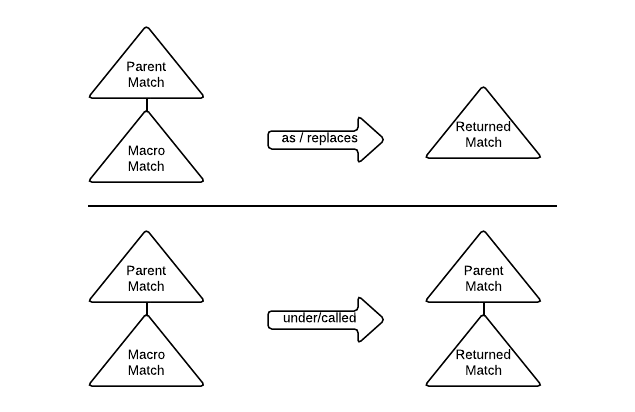
\includegraphics[width=1\textwidth]{img/strats.png}
}
\caption{An illustration of how the different expansion strategies
  work. \texttt{as} differs from \texttt{replaces} by checking that the returned
  match conforms to the parent rule. \texttt{called} differs from \texttt{under}
  by not inserting the macro's rule in the grammar.}
\label{img_strats}
\end{figure}

%%%%%%%%%%%%%%%%%%%%%%%%%%%%%%%%%%%%%%%%%%%%%%%%%%%%%%%%%%%%%%%%%%%%%%%%%%%%%%%%
\subsection{Prioritary Macros}

By default, a macro's rule is inserted as last alternative to its parent
rule. Prioritary macros are instead added as first alternative to their parent
rule. This is sometimes necessary: the only way to write a macro that looks like
a function call is through a prioritary macro.

To make a macro prioritary, add the \texttt{prioritary} keyword right before the
\texttt{macro} keyword, but after the \texttt{raw} keyword, if present.

%%%%%%%%%%%%%%%%%%%%%%%%%%%%%%%%%%%%%%%%%%%%%%%%%%%%%%%%%%%%%%%%%%%%%%%%%%%%%%%%
\section{Working with \texttt{Match}es}
\label{match_api}

This section details the public API of the \texttt{Match} class. Most of the
features relates to finding submatches that fit some criteria.

%%%%%%%%%%%%%%%%%%%%%%%%%%%%%%%%%%%%%%%%%%%%%%%%%%%%%%%%%%%%%%%%%%%%%%%%%%%%%%%%
\subsection{Match Information}

\begin{description}
\item \texttt{originalString()}

  Returns the matched string, exactly like it appeared in the original source.

\item \texttt{string()}

  Returns the matched string, trimmed of leading and trailing
  whitespace. Leading and trailing comments are preserved.

\item \texttt{expression()}

  Returns the \texttt{Expression} this match conforms to.

\item \texttt{children()}

  Returns a \texttt{List<Match>} of the match's children.

\item \texttt{child()}

  Same as \texttt{match.children().get(0)}. Useful when it is known that a match
  has one and only one child.

\item \texttt{empty()}

  Same as \texttt{match.children().isEmpty()}.

\item \texttt{getCaptures(String name)}

  Returns all matches captured with the given name in this match tree, as a
  \texttt{Match[]}. In the body of a macro that has a capture named \texttt{x},
  the variable \texttt{x} is guaranteed to be equivalent to
  \texttt{input.getCaptures("x")}.

  This method is useful to retrieve captures in a rule other than the macro's
  rule.

  If the match this method is called on is itself a capture with the given name,
  it won't be returned.

\end{description}


%%%%%%%%%%%%%%%%%%%%%%%%%%%%%%%%%%%%%%%%%%%%%%%%%%%%%%%%%%%%%%%%%%%%%%%%%%%%%%%%
\subsection{\texttt{MatchSpec}}
\label{matchspec_manual}

A \texttt{MatchSpec} object is a predicate for matches. The
\lstinline{MatchSpec#matches(Match)} method indicates whether the passed match
satisfies the condition expressed by the \texttt{MatchSpec} object.

\texttt{trees.MatchSpec} is actually an abstract class. caxap supplies a few
useful implementation of this class. Each such implementation can be
instantiated either by using its constructor or by using a convenience static
factory method. All implementations are static nested classes of
\texttt{MatchSpec}. All factory methods also belong to \texttt{MatchSpec}.

You can also roll you own implementation of the abstract class.

Here are the supplied implementations. For each we give the signature of its
constructor(s) and the name of the factory method(s). A factory method takes the
same arguments as the associated constructor, and its return type is the
implementing class.

\begin{description}
\item \texttt{StringSpec(String)} / \texttt{rule}

  Matches \texttt{Match} objects for which the result of \texttt{string()}
  equals the supplied string.

\item \texttt{RuleSpec(String)} \& \texttt{RuleSpec(Expression.Rule)} /
  \texttt{rule}

  Matches \texttt{Match} objects for which the result of \texttt{expression()}
  is a rule with the supplied name (\texttt{String} parameter) or with the same
  name as the supplied rule (\texttt{Expression.Rule} parameter).

\item \texttt{ExprSpec(Expression)} / \texttt{expr}

  Matches \texttt{Match} objects for which the result of \texttt{expression()}
  equals the supplied expression.

\item \texttt{OrSpec(MatchSpec...)} / \texttt{or}

  Matches \texttt{Match} object matched by at least one of the supplied specs.

\item \texttt{AndSpec(MatchSpec...)} / \texttt{and}

  Matches \texttt{Match} object matched by all of the supplied specs.

\item \texttt{NotSpec(MatchSpec)} / \texttt{not}

  Matches \texttt{Match} object not matched by the supplied spec.

\item \texttt{HasSpec(MatchSpec)} / \texttt{has}

  Matches \texttt{Match} object which have a descendent that matches the
  supplied spec.

\item \texttt{AnySpec()} / \texttt{anySpec}

  Matches any \texttt{Match} object.

\end{description}

%%%%%%%%%%%%%%%%%%%%%%%%%%%%%%%%%%%%%%%%%%%%%%%%%%%%%%%%%%%%%%%%%%%%%%%%%%%%%%%%
\subsection{Finding Submatches}
\label{finding_submatches}

All methods that search for submatches are passed a \texttt{MatchSpec} as first
parameter. We call it \emph{the main spec}. Only matches fitting this spec can
be returned, although not all fitting matches need to be returned, depending on
the method.

Additionally, one can supply specs for matches that should come to the left or
to the right of the sought matches. We call those specs \emph{left-specs} and
\emph{right-specs}.

We say that a match $A$ is \emph{to the left of} a match $B$ if $A$ is the
descendant of a left-sibling of an ancestor of $B$. A match $A$ comes \emph{to
  the right of} a match $B$ if $A$ is right-sibling of an ancestor of $B$. If
$A$ comes neither to the left or to the right of $B$, meaning one of the two
matches is an ancestor of the other, both matches are said to \emph{overlap}. A
match cannot be at the same time to the left and to the right of another
match. Matches are considered to be ancestors and descendants of themselves.

A depth-first, left-to-right walk of a match tree orders the nodes from left to
right, meaning that no match is visited before all the matches to its left have
been visited, and no match is visited after a match to its right has been
visited. In a depth-first right-to-left walk, nodes are ordered from right to
left. In both cases, all matches are visited, and overlapping matches are
visited in increasing order of depth.

The most general searching methods are \texttt{allBetween(MatchSpec,
  MatchSpec[], MatchSpec[])} and \texttt{allOutside(MatchSpec, MatchSpec[],
  MatchSpec[])}. Those methods return an array of matches. Below we describe the
algorithm used by \texttt{allBetween()}. We then proceed to explain how
\texttt{allOutside()} differs from it, and how all the other searching methods
relate to those two.

\begin{enumerate}

\item Do a depth-first, left-to-right walk of the tree. Test each encountered
  match against the first left-spec. Once a match fits the spec, ignore its
  descendants and test subsequent matches against the second left-spec. Continue
  like this until either all left-specs have been matched, or all the tree nodes
  have been exhausted. In the second case, we stop the algorithm and return the
  empty array. Else we save the location of the match fitting the last left-spec
  (the \emph{left-match}).

\item Do a depth-first, right-to-left walk of the tree. This time we are looking
  for matches fitting the right-specs. Unlike the left-specs, the right-specs
  are iterated from last to first. Like before, if we exhaust the tree nodes, we
  return the empty array, else we save the location of the match fitting the
  first right-spec (the \emph{right-match}).

\item Verify that the right-match comes to the right of the left-match. If not,
  return the empty array.

\item Do a depth-first, left-to-right walk of the tree. Ignore all the matches
  up to the left-match, and all the matches after the right-match. Add all
  encountered matches fitting the main spec to a list of results, and ignore
  their descendants. Return an array containing all the results.

\end{enumerate}

\texttt{allOutside()} works like \texttt{allBetween()}, except that the
left-match is the match fitting the first left-spec and the right-match is the
match fitting the last right-spec (except for the third step). The last step
ignores all nodes between the left-match and the right-match (inclusive). Hence
\emph{outside} instead of \emph{between} in the method name, as that refers to
the parts of the tree where we search for matches fitting the main spec.

The methods \texttt{allAfterFirst(MatchSpec, MatchSpec...)},
\texttt{allBeforeLast(MatchSpec, MatchSpec...)} are like \texttt{allBetween()}
with the second or first array parameter empty, respectively.

Conversely, the methods \texttt{allBeforeFirst(MatchSpec, MatchSpec...)},
\texttt{allAfterLast(MatchSpec, MatchSpec...)} are like \texttt{allOutside()}
with the second or first array parameter empty, respectively.

The method \texttt{all(MatchSpec)} is equivalent to \texttt{allBetween()} with
both array parameters empty. Only the last step is executed, and no matches are
ignored, excepted the descendants of matches fitting the main spec. When both
array parameters to \texttt{allOutside()} are empty, the result is always an
empty array.

All the methods mentioned in this section also have versions in which the words
\texttt{first} or \texttt{last} replace the word \texttt{all} in the method
name. The result of those methods is always equivalent of taking the first or
last item of the array returned by the \texttt{all} version, if not
empty. Otherwise, they returns a value that is recognized by the \texttt{has()}
calls (see next section) as a lack of result.

%%%%%%%%%%%%%%%%%%%%%%%%%%%%%%%%%%%%%%%%%%%%%%%%%%%%%%%%%%%%%%%%%%%%%%%%%%%%%%%%
\subsection{Checking for the Presence of Submatches}

Sometimes, you just want to know whether a match has a submatch fitting a
particular spec. caxap offers three calls towards this end.

\begin{description}

\item \texttt{boolean has(MatchSpec)}

  The simplest one, does as said above.

\item \texttt{boolean has(Match)}

  Takes a \texttt{Match} returned by one of the \texttt{first...()} or
  \texttt{last...()} calls, and checks if the call yielded a result.

\item \texttt{boolean has(Match[])}

  Takes a \texttt{Match} returned by one of the \texttt{all...()} calls, and
  checks if the call yielded some results.

\end{description}

%%%%%%%%%%%%%%%%%%%%%%%%%%%%%%%%%%%%%%%%%%%%%%%%%%%%%%%%%%%%%%%%%%%%%%%%%%%%%%%%
\subsection{Examples}

There are an unlimited amount of ways to combine specs and searching methods to
find matches. Figure \ref{match_finder_examples} shows a few simple examples
extracted from caxap own implementation.

\begin{figure}[here]
\small
\begin{lstlisting}[language=Java, frame=single]
// Get the macro name from its definition.
String ruleName = match.first(rule("identifier")).string();

// Get the macro's parent rule.
String extendedRuleName = match.firstAfterFirst(
    rule("identifier"), rule("strategy")).string();

// Is an unquotation escaped (prefixed by a slash)?
boolean escaped = unquotation.has(
  unquotation.firstBeforeFirst(
    rule("backslash"), or(rule("hash"), rule("hashat"))));
\end{lstlisting}
\caption{Simple examples of submatches finder extracted from caxap
  implementation.}
\label{match_finder_examples}
\end{figure}

%%%%%%%%%%%%%%%%%%%%%%%%%%%%%%%%%%%%%%%%%%%%%%%%%%%%%%%%%%%%%%%%%%%%%%%%%%%%%%%%
\section{(Quasi)quotation}
\label{quotation_manual}

Quotation is one of the basic ways to create new matches in caxap. It is a
process by which we turn some literal source string into a match representing it
as code. Quasiquotation expands on quotation by adding the ability to insert
other fragments of code into our source string.

The design of quasiquotation in caxap follows that of Lisp, with a few
modifications to account for arbitrary syntax. The design of quasiquotation in
Lisp and the evolutions of the concept are thoroughly described in the paper
``Quasiquotation in Lisp''. \cite{quasiquotation}

%%%%%%%%%%%%%%%%%%%%%%%%%%%%%%%%%%%%%%%%%%%%%%%%%%%%%%%%%%%%%%%%%%%%%%%%%%%%%%%%
\subsection{Quotation Basics}
\label{quotation_basics}

\emph{quoting} is the process of turning a character string into a structure
representing code. In our case, this structure is a match tree. Thus quoting is
no different than parsing a source string.

We call \emph{quotation} the application of the \emph{quote} operation. We call
\emph{a quote} the match tree that results from quotation. We use the
\emph{quoted} adjective to refer to the match tree representation of some
code. Quotation takes a source string as input. We call this string \emph{the
  source fragment}.

The example below shows a quoted \texttt{if} statement in caxap. The source
fragment is contained between square brackets. The quotation is delimited by
single quotes. Between the first single quote and square bracket is the name of
the rule used to parse the source fragment (\texttt{expression}).

\begin{lstlisting}
'expression[ if (predicate()) { method(); } ]'
\end{lstlisting}

\emph{Quasiquotation} is similar to quotation, but operates on a source fragment
interspersed with applications of the \emph{unquote} operation
(\emph{unquotation}). The intent of unquotation is to insert some code into a
source fragment. In caxap, said code can be represented by any object, although
we often work with match trees.

The example below shows how to unquote a match for the expression \texttt{42} in
order to obtain a match for the expression \texttt{42 + 52}.

\begin{lstlisting}
Match fortyTwo = 'expression[ 42 ]';
Match sum = `expression[ #fortyTwo + 52 ]`;
\end{lstlisting}

Quasiquotation is delimited by backquotes (\lstinline{`}). The unquotation
operator is the hash symbol (\lstinline{#}). The operator may be followed by any
unary expression, or by another unquotation, which is then said to be nested to
the outer unquotation (see next section). An unary expression is an expression
whose least prioritary operator is not a binary or ternary operator. To use such
operators in conjunction with unquotation, simply wrap the resulting expression
within parentheses. Note that a quotation is a valid unary expression.

The unquotation operand can be any Java object. If it is an instance of
\texttt{Match}, its \texttt{string()} method is used to get the code represented
by the match tree. Otherwise, the \texttt{toString()} method is assumed to
return the represented code.

If the unquotation operand is a match tree, caxap verifies that the unquoted
match tree makes its way to the resulting match tree. This helps avoid scenarios
like this:

\begin{lstlisting}
Match sum = 'expression[ 1 + 1 ]';
Match product = `expression[ #sum * 3 ]`
\end{lstlisting}

\texttt{sum} parses as (1 + 1), whereas \texttt{product} parses as (1 + (1 *
3)), which might not be what we want. The meaning of our code changed because of
the context in which it was inserted.

Admittedly, these checks can be somewhat restrictive. For instance, the
following example won't work because the \texttt{classDeclaration} expected a
\texttt{classBody}, not a \texttt{block}. Normally this is a useful warning: a
class body contains class member declaration and class initializers, whereas a
block contains instructions. Both should not be confused.

\begin{lstlisting}
Match block = 'block [ { int x = 1; } ]';
Match klass = `classDeclaration[ class #block ]`;
\end{lstlisting}

Still, caxap allows you to pull this off very simply should you want it. Simply
convert the match to a string before unquoting it.

\begin{lstlisting}
Match block = 'block [ { int x = 1; } ]';
Match klass = `classDeclaration[ class #block.string() ]`;
\end{lstlisting}

It is also possible to unquote multiple objects at the same time. This is called
splicing and is introduced in section \ref{splicing}.

It may seem that quasiquotation is a generalized form of quotation: quotation is
quasiquotation with no code insertion. Section \ref{non_recur_unquot} shows that
we in fact need both concepts.

We use the terms \emph{quotation}, \emph{quote} and \emph{quoted} to refer to
quotation and quasiquotation both. The context should make clear what is
meant. We sometimes use \emph{simple quotation} to talk about a quotation which
is not a quasiquotation.

Quotations may appear in any source file, not only in macro files. In the
future, I may restrict their use to macro files, unless explicitly requested in
a regular source file.

%%%%%%%%%%%%%%%%%%%%%%%%%%%%%%%%%%%%%%%%%%%%%%%%%%%%%%%%%%%%%%%%%%%%%%%%%%%%%%%%
\subsection{Nested Quotations}
\label{nested_quot}

In addition to being valid operands for unquotations, quotations can also be
quoted. What then should we do in following scenario?

\begin{lstlisting}
`expression[ `expression[ #myExpression ]` ]`
\end{lstlisting}

Assuming \texttt{myExpression} holds a match tree for the code \texttt{1 + 1},
should the returned match tree be for the code \lstinline{`expression[ 1 + 1 ]`}
or for the code \lstinline{`expression[ #myExpression ]`}?

This question shows that we need a way to distinguish unquotations that should
be applied immediately from the ones that should be quoted.

In caxap, the correct answer to the above question is the second one. The
solution to our problem is to use a system of depth. Entering a quasiquotation
(including the top-level one) increases the depth by one, whereas entering an
unquotation decreases it by one. Unquotations entered with a depth of 0 are
applied. Simple quotations do not change the depth, but entering a simple
quotation with depth 0 does prevent the quotations it contains from being
depth-processed.

Figure \ref{quot_ex_one} has an example to help you understand. The arrow
(\texttt{->}) stands for expression evaluation, and \texttt{==} stands for
expression equivalence. The example exhibits the recursive evaluation of an
unquotation's operand: \texttt{y} evaluates to a match tree for \texttt{x},
which itself evaluates to a match tree for \texttt{1}.

\begin{figure}[here]
\small
\begin{lstlisting}[frame=single]
Match x = 'expression[ 1 ]';
Match y = 'expression[ x ]';

   `quotation[ `expression[ ##y ]` ]`
== `quotation[ `expression[ #x ]` ]`
-> `expression[ #x ]`
== `expression[ 1 ]`
-> 1
\end{lstlisting}
\caption{An example that shows the result of recursively evaluating a
  quasiquotation containing nested quotations.}
\label{quot_ex_one}
\end{figure}

While depth-processing a quotation, it is an error if we reach a negative
depth. We always count depth starting at the outermost quotation: nested
quotations are only depth-processed as part of the outermost quotation, never
individually.

Quotations are evaluated within some scope. It is within that scope that the
unquotations with depth 0 are applied. Other unquotations might be applied in
other scopes, if the match tree returned by the quotation gets evaluated in such
a scope. This is typically the case when you compile a match tree to Java code,
then run said Java code. Said otherwise, unquotation operands have a form of
cross-compilation dynamic scope.

%%%%%%%%%%%%%%%%%%%%%%%%%%%%%%%%%%%%%%%%%%%%%%%%%%%%%%%%%%%%%%%%%%%%%%%%%%%%%%%%
\subsection{Non-Recursive Unquotation}
\label{non_recur_unquot}

As you might have noticed, applying a nested unquotation only makes the
innermost unquotation disappear. The unquoted code is still subjected to the
outer unquotations.

Consider then this question. How can obtain a quote for
\lstinline{`expression[ x ]`}, where \texttt{x} is the result of
a method accessible in the current scope?
Consider the following possibilities:

\begin{enumerate}
\item \lstinline{`quotation[ `expression[ ##method() ]` ]`}
\item \lstinline{`quotation[ `expression[ #method() ]` ]`}
\item \lstinline{`quotation[ 'expression[ #method() ]' ]`}
\item \lstinline{`quotation[ 'expression[ #method() ##other() ]' ]`}
\item \lstinline{`quotation[ `expression[ #'expression[ #method() ]' ]` ]`}
\item \lstinline{`quotation[ `expression[ #'expression[x]' ]` ]`}
\end{enumerate}

Item 1 doesn't work: it results in \lstinline{`expression[ #x ]`}. Item 2
doesn't work either: \texttt{method()} is not be evaluated because the
unquotation is entered with depth 1. Item 3 works, but only if the source
fragment does not include other unquotations. This is shown in item 4, which
fails because there is an unquotation with negative depth.

Item 5 is the solution. It is equivalent to item 6. The quotation basically
cancels out the second unquotation by preventing \texttt{x} from being evaluated
later as unquotation operand. After one evaluation, item 4 is therefore
equivalent to \lstinline{`expression[ x ]`}.

This complication is the reason why we need separate notions of quotation and
quasiquotation. The fix exploits the fact that quotation does not increase the
nesting depth.

%%%%%%%%%%%%%%%%%%%%%%%%%%%%%%%%%%%%%%%%%%%%%%%%%%%%%%%%%%%%%%%%%%%%%%%%%%%%%%%%
\subsection{Splicing}
\label{splicing}

Splicing is a variant of unquotation. It allows you to insert an array of
objects in one go. You can specify strings to be inserted before and after the
sequence (unless the sequence is empty), and in-between the items in the
sequence. See the examples in figure \ref{splicing_example}.

\begin{figure}[here]
\small
\begin{lstlisting}[frame=single,language=caxap]
Match[] matches = new Match[] {'expression[ 1 ]', 'expression[ 2 ]'};
Match[] empty   = new Match[] {};

Match args1 = `arguments[ #@ |(|,|)| matches ]`;
Match args2 = `arguments[ ( #@ ||,|| matches ) ]`;

System.out.println(args1.string()); // prints "(1,2)"
System.out.println(args2.string()); // prints "()"
\end{lstlisting}
\caption{caxap code showing example uses of splicing.}
\label{splicing_example}
\end{figure}

The \emph{separators} are enclosed between pipe characters (\texttt{|}). The
first one goes before the sequence, the last one after, and the middle one in
between each item. Any of them can be omitted. If the spliced array is empty,
nothing is inserted.

The spliced object must be an array, but can be any type of array. Each item in
the array is handled as in regular unquotation. This means that even in an
\texttt{Object} array, the code for a \texttt{Match} is obtained by calling its
\texttt{string()} method, and that there are checks to make sure that an
equivalent match makes it to the resulting tree.

If you want to bypass those checks, the static method \texttt{String[]
  Match.strings(Object[])} will convert an array of objects to an array of
\texttt{String} for you. This array can then be spliced with equivalent results
as splicing the original array, except for the checks.

See section \ref{quotation_basics} for all the details about regular
unquotation.

%%%%%%%%%%%%%%%%%%%%%%%%%%%%%%%%%%%%%%%%%%%%%%%%%%%%%%%%%%%%%%%%%%%%%%%%%%%%%%%%
\subsection{Quotation \& Escaped Sequences}

We have now seen all syntaxes for quotation. Those syntaxes are delimited by
some special characters or character sequences. This means there are places
where you can't use those characters or sequences. You can however substitute
them with the escaped sequences described in this section.

In both regular quotations and quasiquotations, the sequences \lstinline{]'} and
\lstinline{]`} cannot appear. They can however appear as part of a unary
expression which is part of an unquotation, and should not be escaped there. To
escape those sequences, simply prefix them with a backslash (\lstinline{\}). If
  you want to end your source fragment by a backslash, you should make sure that
  your rule allows trailing whitespace, and put some whitespace between your
  backslash and the closing square bracket. In the base Java grammar, all rules
  that can end with a backslash allow trailing whitespace.

  The hash character can also be escaped inside quotations by prefixing it with
  a backslash: \lstinline{\#}. To have an unquotation preceded by a backslash,
  use the whitespace trick mentioned above: \lstinline{\ #}.

  Note that those escapes must appear even in unlikely places, such as string
  literals. You however never have to worry about escaping a Match that is
  handed to you from some other source. You only have to worry about escaping
  when writing things inside the brackets of the quotation syntax.

  When using the splice operator, you can escape the pipe character with
  \lstinline{\|}. The backslash character must itself be escaped:
  \lstinline{\\}. We also support some additional escapes for convenience:
  \lstinline{\t} for tabulation, \lstinline{\n} for newline, and \lstinline{\r}
  for carriage return. For implementation reasons, other backslash-prefixed
  escapes might also work, but there is no guarantee that they will remain
  supported. There are not needed anyway.

  Finally, it should be noted that it is not possible to use quasiquotation to
  quote some code with significant leading whitespace: that whitespace gets
  consumed by the \texttt{[} token in the quotation syntax. Note that whitespace
  includes comments. There is a workaround: just output the whitespace to a
  string, and unquote that string at the begin of the quotation (make it a
  quasiquotation if needed). This workaround is demonstrated in the file
  \texttt{examples/src/pkg/Comments.javam}.

%%%%%%%%%%%%%%%%%%%%%%%%%%%%%%%%%%%%%%%%%%%%%%%%%%%%%%%%%%%%%%%%%%%%%%%%%%%%%%%%
\section{Macro Composition}

Up to this point, we have explained how macros work in isolation. This section
examines how macros can interact with each other.

%%%%%%%%%%%%%%%%%%%%%%%%%%%%%%%%%%%%%%%%%%%%%%%%%%%%%%%%%%%%%%%%%%%%%%%%%%%%%%%%
\subsection{Composing Unrelated Macros}

% TODO until

Consider the \texttt{Unless} macro from figure \ref{simple_macro_example} and
the \texttt{Until} macro from figure \ref{until_macro}. Each macro has
\texttt{statement} as parent rule, and can have statements as submatches, via
the \texttt{block} rule. caxap naturally allows an \texttt{Unless} match to be a
submatch of an \texttt{Until} match, and vice-versa. In fact an \texttt{Until}
match can perfectly be a submatch of another \texttt{Until} match. The point is
illustrated in figure \ref{composition_example}.

\begin{figure}[here]
\small
\begin{lstlisting}[frame=single,language=caxap]
macro Unless as statement
: "until" expr:expression :block {
  return `statement[ while (!(#expr[0])) #block[0] ]`;
}
\end{lstlisting}
\caption{caxap code defining an \emph{unless} construct (a while loop with a
  negated condition) as a macro.}
\label{until_macro}
\end{figure}

\begin{figure}[here]
\small
\begin{lstlisting}[frame=single,language=Java]
int i = 0;
until i == 10 {
  unless i % 2 == 0 {
    System.out.println(i);
  }
}
\end{lstlisting}
\caption{Composing the \texttt{Unless} and \texttt{Until} macros. The code
  prints all odd number between 0 and 10.}
\label{composition_example}
\end{figure}

Because arbitrary code can be run to generate a macro's expansion, it cannot be
guaranteed that all macros can be freely composed. Macro implementers should be
loath to introduce such incompatibilities, and if they really have to, should
clearly document them.

%%%%%%%%%%%%%%%%%%%%%%%%%%%%%%%%%%%%%%%%%%%%%%%%%%%%%%%%%%%%%%%%%%%%%%%%%%%%%%%%
\subsection{Macro Expansion Order \& Raw Macros}
\label{raw_macros}

Macros are expanded bottom-up. This means that in figure
\ref{composition_example}, the \texttt{Unless} macro call will be expanded
before the \texttt{Until} macro call.

In the case of figure \ref{composition_example}, this distinction is irrelevant:
since the statements submatches are copied to the output, the \texttt{Unless}
macro call would have been expanded after the \texttt{Until} call if macros
weren't expanded bottom-up (because of recursive expansion, as explained in
section \ref{macro_expansion_intro}).

Sometimes order matters, or you don't want a macro to expand to all.  In those
cases, you can use \emph{raw macros}. A raw macro is a macro whose macro
submatches are not expanded. You can then pass them on to the output, which will
cause them to expand, or just ignore them. You make a macro raw by prefixing its
definition with the \texttt{raw} keyword.

%%%%%%%%%%%%%%%%%%%%%%%%%%%%%%%%%%%%%%%%%%%%%%%%%%%%%%%%%%%%%%%%%%%%%%%%%%%%%%%%
\subsection{Macros Referencing Macros}
\label{noop_macros}

A macro's syntactic declaration can contain direct references to other macros'
rules - or in fact, to their own rule - as long as those rule use the
\texttt{called} expansion strategy. This is currently not enforced by caxap: the
checks need to be implemented. The macros must have been required - or defined
earlier in the same file - in order to be referencable.

For macro with the \texttt{called} strategy, you can elect to replace the macro
body by a semicolon. The resulting macros are called \emph{no-op macros} and do
not expand: the match is preserved as though it was under a raw macro. This
allows you to define reusable syntactic elements.

A macro's parent rule can also be another macro's rule. Albeit we do not
currently restrict this, extending a macro which is not no-op is fraught with
peril. You risk causing an error in the parent macro's expansion code, which
more than likely references the matched input.

%%%%%%%%%%%%%%%%%%%%%%%%%%%%%%%%%%%%%%%%%%%%%%%%%%%%%%%%%%%%%%%%%%%%%%%%%%%%%%%%
\section{Error Reporting}
\label{error_reporting_manual}

Error reporting in caxap is currently in a poor state. In case of error, you
should in principle get a message describing exactly what went wrong and caused
caxap to abort, but the details may sometimes be vague. You'll also get a nice
Java stack trace for free.

Currently, most errors are implemented as unchecked exception that bubble up to
the top of the call stack. In the future, I plan to consolidate all the
exceptions in a well thought-out hierarchy.

A special note on syntax errors: arbitrary syntax makes them especially
difficult to get right.

Parse errors are normal during PEG parsing: they simply mean that we should try
the next alternative of an ancestor of the failing expression. When all possible
alternatives fail, the whole parse fails and we should report a syntax error.

The current strategy is to keep track of the farthest input position causing an
error. Once there are no more alternatives to try, we report all errors at that
farthest input position.

Surprisingly, there can be quite a few different errors happening at the same
input position, and caxap currently display the ancestry of all of them. This
can make the output of a parse error quite unwieldy.

caxap already has some tricks to lessen the information overload. For instance,
if a rule fails without matching any character, only the name of that rule is
reported, and not all of its alternatives, which by definition also failed.

Error reporting for grammars which are not fixed in advance is known to be a
hard problem, and other generic PEG parsers such as Parboiled \cite{parboiled}
or Mouse \cite{redziejowski2009} don't do better than caxap in this regard.

%%%%%%%%%%%%%%%%%%%%%%%%%%%%%%%%%%%%%%%%%%%%%%%%%%%%%%%%%%%%%%%%%%%%%%%%%%%%%%%%
\section{Miscellaneous Concerns}

If you choose to reference the grammar rule for macro definition
(\texttt{macroDefinition}) from your own macro, you must make sure that if a
macro definition is parsed, it will make it to the final match tree. The reason
for this constraint is explained in section \ref{implem_grammar}.

You can use caxap's API in your regular programs (i.e. outside of macros). But
if you do so, you need to make sure that caxap's jar file appears on the
classpath of your program.

A common pattern in macro development is to factor out some common logic between
macros to an external class. Unfortunately this class will be expanded and
copied to the output directory like the rest. When you try to compile it, Java
will serve you an error if caxap is not on your classpath. This will be fixed in
a future release.
